\documentclass[conference]{IEEEtran}
\IEEEoverridecommandlockouts
% The preceding line is only needed to identify funding in the first footnote. If that is unneeded, please comment it out.
\usepackage{cite}
\usepackage{amsmath,amssymb,amsfonts}
\usepackage{algorithmic}
\usepackage{graphicx}
\usepackage{textcomp}
\usepackage{xcolor}
\usepackage{amssymb}
\usepackage[normalem]{ulem}
\useunder{\uline}{\ul}{}
\def\BibTeX{{\rm B\kern-.05em{\sc i\kern-.025em b}\kern-.08em
    T\kern-.1667em\lower.7ex\hbox{E}\kern-.125emX}}

\title{CalBERT -- Code-mixed Adaptive Language representations using BERT
}


\makeatletter
\newcommand{\linebreakand}{%
  \end{@IEEEauthorhalign}
  \hfill\mbox{}\par
  \mbox{}\hfill\begin{@IEEEauthorhalign}
}
\makeatother

\author{
  \IEEEauthorblockN{Aditeya Baral}
  \IEEEauthorblockA{\textit{Dept. of CSE} \\
    \textit{PES University}\\
    Bengaluru, India \\
    aditeya.baral@gmail.com}
  \and
  \IEEEauthorblockN{Ansh Sarkar}
  \IEEEauthorblockA{\textit{Dept. of CSE} \\
    \textit{PES University}\\
    Bengaluru, India \\
    anshsarkar1@gmail.com}
  \and
  \IEEEauthorblockN{Aronya Baksy}
  \IEEEauthorblockA{\textit{Dept. of CSE} \\
    \textit{PES University}\\
    Bengaluru, India \\
    abaksy@gmail.com}
  \linebreakand % <------------- \and with a line-break
  \IEEEauthorblockN{Deeksha D}
  \IEEEauthorblockA{\textit{Dept. of CSE} \\
    \textit{PES University}\\
    Bengaluru, India \\
    deekshad132@gmail.com}
  \and
  \IEEEauthorblockN{Prof. Ashwini M Joshi}
  \IEEEauthorblockA{\textit{Dept. of CSE} \\
    \textit{PES University}\\
    Bengaluru, India \\
    ashwinimjoshi@pes.edu}
}
\begin{document}

\maketitle

\begin{abstract}
A code-mixed language is a type of language that involves the combination of two or more language varieties in its script or speech. Code-mixed language has become increasingly prevalent in recent times, especially on social media. However, the exponential increase in the usage of code-mixed language, especially in a country like India which is linguistically diverse has led to various inconsistencies. Analysis of text is now becoming harder to tackle because the language present is not consistent and does not work with predefined existing models which are monolingual. We propose a novel approach to improve performance in Transformers by introducing an additional step called "Siamese Pre-Training", which allows pre-trained monolingual Transformers to adapt language representations for code-mixed languages with a few examples of code-mixed data. Our studies show that CalBERT is able to improve performance over existing pre-trained Transformer architectures on downstream tasks such as sentiment analysis. Multiple CalBERT architectures beat the state of the art $\mathbf{F_1}$-score on the Sentiment Analysis for Indian Languages (SAIL) dataset, with the highest possible improvement being 5.1 points. CalBERT also achieves the state-of-the-art accuracy on the IndicGLUE Product Reviews dataset by beating the benchmark by 0.4 points.
\end{abstract}

\begin{IEEEkeywords}
code-mixed languages, Transformer, BERT, SAIL, sentiment analysis
\end{IEEEkeywords}

\section{Introduction}
Code-mixed language\cite{b1} is a form of language wherein syntactic elements from one language (such as words, phrases or even sentences)  are inserted into another language in such a way that the semantics of the resultant language remain the same. Code-mixed language is more prevalent in a multilingual society like India, where most of the population are bi-lingual, if not more than that. This code-mixed language is most prevalent on social media platforms such as Facebook and Twitter. Given the interest of enterprises in determining business insights from social media posts, generating a mechanism for the proper analysis, and understanding of code-mixed language gains even more importance. 

One of the primary tasks in natural language processing is building a language representation for a given natural language. These language representations are used to adapt learning models for specific natural language understanding tasks like sentiment analysis and human-like conversation systems. Language representations have been built using various statistical and deep learning techniques, with the current state of the art methods employing Transformer architectures pre-trained on vast amounts of natural language data to learn these representations. However, almost all of these learnt representations are monolingual and have been created using a single language only, or pre-trained on multiple languages individually. These representations struggle when a language might be code-mixed and hence display low performance on code-mixed natural language tasks due to inherent inconsistenices and large variability in data.

Our novel approach generates Code-mixed Adaptive Language representations using Bidirectional Encoder Representations from Transformers (CalBERT) by adding an additional pre-training step called "Siamese Pre-Training" where a pre-trained monolingual Transformer\cite{b2} is provided with different representations of the same sentence or phrase and learns to minimise the distance between their embeddings. We evaluate CalBERT on sentiment analysis\cite{b4} of the Hinglish language using the benchmark SAIL 2017 dataset\cite{b5} and obtain an $F_1$-score of 62\%, thus obtaining an improvement of 5.1 points, or 8.9\%. We also evaluate CalBERT on the sentiment analysis task released by IIT Patna using the IndicGLUE Product Reviews dataset\cite{b17}, and obtain an accuracy of 79.37\%,  a 0.5\% increase over the existing benchmark. 

\section{Background}

BERT\cite{b6} and similar transformer architectures derived from BERT (such as RoBERTa\cite{b7}, DistilBERT\cite{b8} and others) are used to extract language representations from text corpora. These language representations are learned using a bidirectional attention mechanism\cite{b9}, and incorporate contextual information about the individual tokens in the corpus, and can be fine-tuned for a variety of tasks in natural language understanding. The large majority of existing models that are based on BERT and BERT-like architectures are trained on monolingual text corpora, and as such, produce representations that are more attuned for high performance in tasks involving a single language. As such, these representations suffer from poor performance when applied to natural language understanding tasks involving code-mixed language that contains multiple language varieties in a single script language. 
The methodology proposed in this work seeks to adapt existing representations for monolingual text into representations that can be fine-tuned for tasks in code-mixed languages. This allows for representations of code-mixed language to be generated without having to pre-train an empty Transformer model from scratch on large quantities of code-mixed data, which is a time consuming and computationally intensive process. 

\section{Previous Work}

Mikolov, in his paper titled “Efficient Estimation of Word Representations in Vector Space”\cite{b10}, proposes an novel approach to compute word embeddings without the added complexity of a hidden layer while performing better than neural network language model. These word vectors outperform the SemEval 2012 task-2 benchmark however perform poorly on out of vocabulary words and morphologically rich languages. 

Reimers et al, in their work titled “Sentence-BERT: Sentence Embeddings using Siamese BERT-Networks”\cite{b11} modify the existing BERT architecture to use a Siamese network with shared weights and cosine similarity as the loss function to predict the semantic textual similarity. The model was able to train in linear time yields a score of 84.88\% in sentiment prediction of movie reviews. 

“A Passage to India: Pre-trained Word Embeddings for Indian Languages"\cite{b12} by Kumar et al, shows that models trained on sub word representations perform better as Indian languages are morphologically rich. Their multilingual embeddings when evaluated on next sentence prediction using pre-trained BERT gives 67.9\% accuracy. Another paper titled “Towards Sub-Word Level Compositions for Sentiment Analysis of Hindi-English Code Mixed Text”\cite{b13} by Joshi et al, discusses the advantage of using sub word representations compared to character level tokens to deal with inconsistencies in code-mixed text. This method was evaluated on a custom dataset and yields an $F_1$-score of 65.8\%.

Choudhary et al\cite{b14}, in their paper “Sentiment Analysis of Code-Mixed Languages leveraging Resource Rich Languages” propose a novel method which uses contrastive learning. They use a Siamese model to map code-mixed and monolingual language to the same space by clustering based on similarity between their skip-gram vectors. This works on the hypothesis that similar words have similar contexts. The model achieves 75.9\% F-score on the HECM dataset, an improvement over existing approaches.


\section{Proposed Approach}
We propose a novel approach to adapt Transformer representations for a code-mixed language from existing representations that exist in another language by introducing an additional pre-training step using a Siamese network architecture\cite{b3}. We attempt to minimise the distance between the two semantic spaces of the corresponding languages and obtain a joint or shared representation for equivalent sentences in both languages. This additionally enables the generation of code-mixed language representations from an existing language's representations, without the need to pre-train a Transformer from scratch, which is computationally expensive.

Our novel approach is implemented by using a shared pre-trained Transformer layer in each of the branches of the Siamese network and use an appropriate loss function to bring the embeddings closer between each pair of sentences. To Siamese-pretrain CalBERT, the same sentence needs to be obtained in both the language that the Transformer was pre-trained in, along with the language for which the Transformer is trying to adapt representations.

\section{Methodology}

\subsection{Terminologies}

The following terms have been used extensively in the paper.

\begin{itemize}
\item \textit{Base Language}: The single language that was used to pre-train the Transformer architecture. Could be any task like Masked Language Modelling\cite{b6}, Next Sentence Prediction and so on. For example, in the case of the Hinglish language the base language is English.
\item \textit{Target Language}: The code-mixed language for which the Transformer architecture is trying to adapt representations. This language is a super-set of the base language, since it may contain sentences entirely in the base language. For example, Hinglish.
\item \textit{Siamese Pre-training}: The novel additional pre-training step proposed to adapt representations.
\end{itemize}

\subsection{Siamese Pre-training}

% insert img here SBERT
\begin{figure}
    \centering
    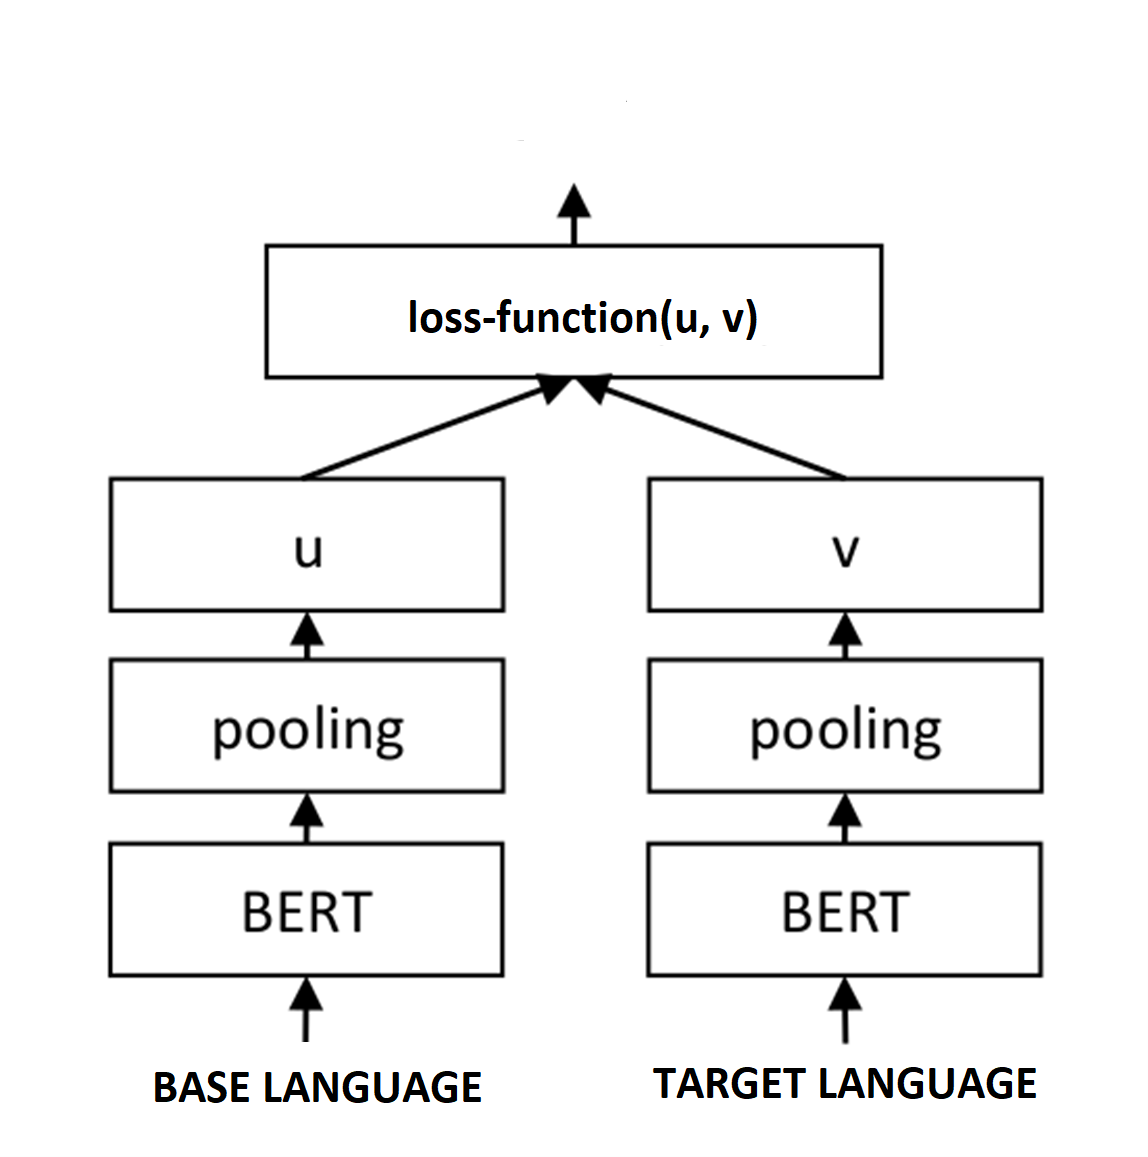
\includegraphics[scale=0.35]{img/sbert-architecture.png}
    \caption{SBERT Architecture used for Siamese Pre-training}
    \label{fig:my_label}
\end{figure}

A Siamese network is a network consisting of two or more branches, wherein each branch receives an input. The network learns to distinguish between the examples provided through each branch. Siamese networks have been used extensively in computer vision for image classification.

A pre-trained monolingual Transformer being trained on only a single language is capable of generating language representations for that langauge only, thus performing poorly when the language is code-mixed. Pre-training a Transformer from scratch on code-mixed data is a difficult task, since it is computationally expensive and also time consuming. Since the Transformer has learnt language representations for one of the languages, it is far more optimal to adapt these existing representations for new and similar words belonging to the other language.

A pre-trained monolingual Transformer is provided with different representations of the same sentence or phrase and learns to minimize the distance between their embeddings (Fig. \ref{fig:my_label}). The two representations in this case are the transliterated version of the code-mixed sentence in the target language, and the translated version in the base language. Since the two versions have the same semantic meaning, their similarity should ideally be as high as possible and thus the distance between their representations should be minimum. Since the Transformer already knows representations for the base language, it only needs to adapt representations to map the target language to the same space. 

The Siamese pre-training is called thus because of its use of the Siamese network architecture, wherein the two arms of the network are fed with two semantically equivalent input sentences in the base and the target language respectively. The network learns the embeddings for both sentences by comparing their similarity (normally, this involves the use of a labelled dataset with sentence pairs and the corresponding similarities, but here all the sentence pairs have maximum similarity). The loss function (Eqn. \ref{cosine-sim} and \ref{contrastive}) used here is used to bring the representations from the two branches closer. In our work we use the cosine distance as the loss function, although similar loss functions such as contrastive loss can also be used. Minimizing the cosine distance implies that the similarity is maximized between the two sentence embeddings, which is the desired outcome. 

The Siamese pre-training is performed as the last pre-training step (after the usual pre-training strategies used in a Transformer such as masked language modelling or next sentence prediction), since it needs existing base language representations to learn the target language effectively. Additionally, our work shows that a significant amount of data is not required to effectively perform Siamese pre-training and that the model is able to learn with a fraction of the data size that was used for pre-training, thus showing that our approach does not require vast computational resources to improve performance.

A variety of BERT-based architectures were pre-trained and fine-tuned for the purposes of this work. The models that were evaluated were BERT, RoBERTa and DistilBERT. These three architectures are used either pre-trained on an English corpus (as available publicly on the HuggingFace Hub), or pre-trained on the corpus of code-mixed data that was collected as part of this experiment.

\section{Workflow}
We focus our efforts on Transformer architectures based on the Bidirectional Encoder Representations from Transformers (BERT) architecture, since they are bidirectional models capable of learning representations from a given sequence using both forward as well as backward context. We demonstrate our novel approach on the Hindi-English (Hinglish) code-mixed language and data for the same was obtained from social media and news articles to maintain a good balance of well structured as well as informal code-mixed language usage. 

\subsection{Equations}
The objective is to minimize the distance between the representation in the base language and the representation in the target language. The loss function, hence, needs to reflect this minimization of the distance between the two representations.\\

The cosine distance loss function in \eqref{cosine-sim} represents the angle between two vectors. Minimzing the cosine distance implies that the two vectors are highly similar as a smaller angle between the two vectors creates a smaller cosine distance. 
\begin{equation}
\label{cosine-sim}
    l(\overrightarrow{a}, \overrightarrow{b}) = \frac{\overrightarrow{a} . \overrightarrow{b}}{\lVert\overrightarrow{a}\rVert \lVert  \overrightarrow{b}\rVert}
\end{equation}

The contrastive loss function takes the output for a positive example and computes its distance to an example of the same class, and then contrasts that with the distance to negative examples. 

\begin{equation}
\label{contrastive}
    l(\overrightarrow{a}, \overrightarrow{b}) = -log \left ( \frac{exp(sim(\overrightarrow{a}, \overrightarrow{b})/ \tau)}{\sum\limits_{k=1}^{2N} exp(sim(\overrightarrow{a}, \overrightarrow{b})/ \tau)} \right )
\end{equation}

Here, $N$ is the total number of examples and $\tau$ is a temperature normalization factor. $sim(\overrightarrow{a}, \overrightarrow{b})$ represents the similarity metric between the embedding vectors $\overrightarrow{a}$ and $\overrightarrow{b}$ which is used to appropriately train the positive and negative examples. Metrics such as cosine similarity can be used for this application. \\

The online contrative loss function is similar to contrastive loss as shown above, but it selects hard positive (positives that are far apart) and hard negative pairs (negatives that are close) and computes the loss only for these pairs. This approach is often found to yield better performance than contrastive loss.



\subsection{Data Collection}
Since code-mixed Hinglish data is abundantly present on platforms like social media, we choose to use social media as our source of data. Platforms like Twitter and Facebook were scraped and compiled together. There are also several online archives available which host code-mixed data for several tasks. Additionally, Hinglish code-mixed data is already available on IndicCorp, which is one of the largest publicly-available corpora for Indian languages. 

After compiling all the sources of data together, they need to be converted into a suitable pairwise format to be used along with CalBERT. 
\subsection{Data Preprocessing}

Although a large amount of data is obtained (Table \ref{tab:calbert_dataset_metrics}), most of it is not in a format that can be directly used to train CalBERT. Since Hinglish code-mixed language can exist in both the Hindi (Devanagiri) script as well as Roman script, we need to transliterate all of them to the same single script language. For our work, we choose the script language to be Roman since most popular Transformer architectures have been pre-trained in this script language, and hence have representations for the base language, in our case English.

For code-mixed data that already exists in the Roman script, we need to obtain the translated version of the same for the base language representation. This has been performed by using software automation tools such as Selenium combined with Google Translate. Alternatively, for code-mixed data that exists in the Devanagiri script, we employ the use of a transliteration library and convert them into the ITRANS ASCII transliteration scheme\cite{b15}.

The input to CalBERT consists of sentence pairs (Table \ref{tab:calbert_data_format}). Each pair consists of the transliteration of the code-mixed sentence in the target language, and the translation of the same code-mixed sentence in the base language. Both sentences are represented in the Roman script in our work. Since both sentences have the same semantic meaning, the objective is to reduce the distance between the corresponding sentence representations. The shared Transformer layer in CalBERT thus allows it to learn joint representations for both languages and adapts base language representations to the target language.

Due to computational limitations, we did not Siamese pre-train our models on the data obtained from IndicNLP\cite{b16}. However, our experiments show that the small portion of data obtained via scraping was able to boost performance significantly.


\begin{table}[htbp]
    \centering
    \caption{CalBERT Dataset Metrics}
    \label{tab:calbert_dataset_metrics}
    \begin{tabular}{|c|c|}
        \hline
        \textbf{Source} & \textbf{Number of sentences}  \\
        \hline 
        Social Media & 147731 \\
        \hline 
        IndicNLP & 8466307 \\
        \hline
    \end{tabular}
\end{table}

\begin{table}[htbp]
\caption{Base and target language pairs used to train CalBERT}
\label{tab:calbert_data_format}
\begin{center}
    \begin{tabular}{|p{0.2\textwidth}|p{0.2\textwidth}|}
    \hline
    \textbf{Base Language} & \textbf{Target Language} \\
    \hline
    in reply, pakistan got off to a solid start &   jisake javaba mem pakistan ne achchi shuruata ki thi.\\
    \hline
    by this only, we can build our country and make it great again & isake jariye hi hama desha ka nirmana karemge aura use mahana bana payemge \\
    \hline
    people started gathering & logom ki bhida jama hone lagi \\
    \hline
    obtain loans from a bank or an individual & kisi bank ya vyakti se rrina prapta kara sakati hai \\
    \hline 
    he was later taken to a hospital and treated & bada mem use aspatala le jaya gaya aura ilaja kiya gaya \\
    \hline
    a police investigation into the matter is currently underway & aise mem abhi police jamcha ki ja rahi hai \\
    \hline
    money is not that important & dhana adi padartha koi mahatva ki vastue nahim haim \\
    \hline
    i love watching tennis. &  mujhe tennis dekhane ka shauka hai \\
    \hline
    ive always done everything i could to represent my country & maimne hamesha apane desha ka pratinidhitva karane ka prayasa kiya hai\\
    \hline
    arjun kapoor is the son of the famous producer, boney kapoor.  & arjun kapoor film industry ke famous producer boni kapur ke bete haim \\
    \hline
    children are considered to be gifts from god & bachche bhagavana ka rupa mane jate haim \\
    \hline
    it's our cultural heritage & yaha hamari samskrritika virasata hai \\
    \hline 
    no injuries have been reported so far, said a police official & police ka adhikarika taura para kahana hai abhi taka kisi ke gambhira rupa se ghayala hone ki khabara nahim hai \\
    \hline 
    the doctor gave her a massive dose of morphine and put her to sleep again.   &   daktara ne use morphine ki eka ba.di khuraka di aura phira se sula diya \\
    \hline
    he was later arrested and subsequently released from jail & unhem jail mem bamda kiya gaya tha aura bada mem riha kara die ga \\
    \hline
    \end{tabular}
    \label{tab1}
    \end{center}
\end{table}


\subsection{Evaluation Metric}
Since CalBERT is trained in a task-agnostic manner, it can be fine-tuned on any downstream natural language understanding task like sentiment analysis and question answering. We evaluate CalBERT on the Sentiment Analysis for Indian Languages (SAIL) 2017 dataset, which consists of Hinglish code-mixed data in the Roman script. 

The dataset serves as a good evaluation strategy, since it has been compiled with data from various sources ranging from news articles to even social media and consists of various code-mixed forms for the same word and is often considered a difficult dataset to perform well on. It also serves as a benchmark dataset for sentiment analysis on Hindi-English and Bengali-English data, with the highest possible $F_1$-score achieved on the dataset being 56.9\%.

We also evaluate CalBERT on the IndicGLUE Product Reviews dataset released by IIT Patna, which serves as another benchmark dataset for sentiment analysis of Hinglish text, but in the Hindi (Devanagiri) script. All models evaluated on this script have either been trained on English scripted text, or on Devanagiri scripted text. We however propose to evaluate CalBERT on a code-mixed version of the dataset by transliterating the text from Devanagiri to Roman.

The dataset is popularly used for evaluating the performance of Transformers built for Indian languages such as IndicBERT and consists of reviews for products across various categories. The highest possible $F_1$-score obtained on this dataset by IndicBERT is 71.32\%.

\subsection{Siamese Pre-training CalBERT}
% add reference to SBERT library
To Siamese pre-train a Transformer (Table \ref{tab:hyperparam_table}), we first initialise a Siamese network with a shared layer containing the Transformer whose representations we intend to adapt (BERT, RoBERTa or DistilBERT). This can be done effectively using a sentence-transformer architecture. We add a single pooling layer to each branch, and then finally combine the pieces together by adding a suitable loss function to reduce the distance between the representations. In our preliminary experiments, we observe that the contrastive and cosine distance loss functions perform nearly the same and hence use the cosine distance loss function for all the experiments performed. This shared Transformer layer can then be extracted and fine-tuned on other downstream tasks.
 
\begin{table}[htbp]
    \centering
    \caption{Hyperparameters for Siamese Pre-training}
    \label{tab:hyperparam_table}
    \begin{tabular}{|c|c|}
        \hline
        \textbf{Hyperparameter} & \textbf{Value}  \\
        \hline 
        Number of epochs & 10 \\
        \hline 
        Number of warm-up steps & 100 \\
        \hline 
        Learning Rate & $2.5 \times 10^{-5}$ \\
        \hline 
        Weight decay & 0.01 \\
        \hline 
        Optimizer & AdamW \\
        \hline 
        Maximum gradient normalization & 1.0 \\
        \hline 
    \end{tabular}
\end{table}

\section{Evaluating CalBERT}

CalBERT is meant to be fine-tuned for downstream tasks involving code-mixed data. Due to the abundance of code-mixed Hinglish data available on social media and the much need for code-mixed Transformer architectures, we evaluate performance on the popular downstream task of sentiment analysis. 

\subsection{SAIL 2017}

The Sentiment Analysis of Indian Languages (SAIL) 2017 dataset is a collection of sentences in two popular Indian code-mixed languages -- Hindi-English and Bengali-English. The datasets are composed of sentences from various sources like news articles as well as social media and are in the Roman script. There is also a high degree of variability in the data, with multiple forms existing for the same word and different styles of writing. The sentences are classified into 3 polarities -- positive, neutral and negative. The SAIL 2017 task is a challenging benchmark, and is widely regarded as one of the benchmark datasets for sentiment analysis of the Hinglish language. The highest documented $F_1$-score on the benchmark is 56.9\%.

\begin{table}[htpb]
    \centering
    \caption{SAIL 2017 Dataset Metrics}
    \label{tab:sail_dataset}
    \begin{tabular}{|c|c|}
    \hline 
        \textbf{Dataset Split} & \textbf{Number of examples} \\
    \hline
        Train set & 9945 \\
    \hline
        Test set & 1238 \\
    \hline
        Validation set & 1240 \\
    \hline
    \end{tabular}
\end{table}

The SAIL 2017 dataset is already partitioned into train, test and validation splits (Table \ref{tab:sail_dataset}). All comparisons are made using the $F_1$ score on the validation split. For our experiments, we fine-tune existing pre-trained models with and without CalBERT's additional Siamese pretraining step and compare the score obtained by each model. The experiments are performed multiple times using the same set of hyperparameters and the highest $F_1$-score over 10 runs is recorded.

\begin{table}[htbp]
    \centering
    \caption{Hyperparameters for SAIL 2017 Fine-Tuning}
    \label{tab:finetuning_hyperparams}
    \begin{tabular}{|c|c|}
    \hline
        \textbf{Hyperparameter} & \textbf{Value}  \\
    \hline
        Learning Rate & $2 \times 10^{-6}$ \\
    \hline 
        Training Batch Size & 4 \\
    \hline 
        Evaluation Batch Size & 4 \\
    \hline 
        Number of epochs & 15 \\
    \hline 
        Weight Decay & 0.08 \\
    \hline
    \end{tabular}
\end{table}

CalBERT outperforms the SAIL 2017 benchmark (Table \ref{tab:results_calbert}) $F_1$-score by 5.1 points, or 8.9\% with the CalBERT-XLM-RoBERTa model (XLM-RoBERTa with CalBERT's Siamese pre-training). We also improve upon on the benchmark precision by 3.5\% and the recall by 10.3\%. Additionally, all other CalBERT architectures also outperform the benchmark $F_1$-score, with the minimum improvement obtained by CalBERT-DistilBERT being 3\%.

\begin{table}[htbp]
\centering
\caption{Comparison of $F_1$-scores on SAIL 2017 benchmark}
\label{tab:results_calbert}
\begin{tabular}{|p{0.16\textwidth}|p{0.05\textwidth}|p{0.07\textwidth}|p{0.05\textwidth}|}
\hline
\textbf{Model Type} & \textbf{$F_1$-Score} & \textbf{Precision} & \textbf{Recall}\\ 
\hline
\textbf{CalBERT-XLM-RoBERTa} & \textbf{\textcolor{red}{0.620}} & \textcolor{red}{\textbf{0.618}} & \textcolor{red}{\textbf{0.618}} \\ 
\hline
CalBERT-RoBERTa & \textcolor{red}{0.612} & \textcolor{red}{0.615} & \textcolor{red}{0.614} \\
\hline
CalBERT-BERT & \textcolor{red}{0.588} & 0.581 & \textcolor{red}{0.583}  \\ 
\hline
CalBERT-DistilBERT  & \textcolor{red}{0.586} & 0.587 & \textcolor{red}{0.586} \\
\hline
CalBERT-IndicBERT & 0.530 & 0.529 & 0.531 \\
\hline
\textbf{SAIL-2017   Benchmark} & \textbf{0.569}  & \textbf{0.597} & \textbf{0.56} \\ \hline
\end{tabular}
\end{table}

\begin{table}[!h]
    \centering
    \caption{Confusion Matrix for CalBERT-XLM-RoBERTa Model (SAIL)}
    \label{tab:confusion_matrix}
    \begin{tabular}{|c|c|c|c|}
    \hline
        & \textbf{Negative} & \textbf{Neutral} & \textbf{Positive} \\
    \hline
        \textbf{Negative} & 148 & 93 & 41 \\
    \hline
        \textbf{Neutral} & 80 & 359 & 124 \\
    \hline
        \textbf{Positive} & 44 & 92 & 259 \\
    \hline
    \end{tabular}
    
\end{table}

We observe that Transformer architectures also obtained improved performance metrics on the SAIL 2017 benchmark. For this reason we evaluate CalBERT's Siamese pre-training against a native Transformer that was used to Siamese pre-train CalBERT (Table \ref{tab:calbert_influence_results}). Our experiments show that CalBERT has improved the $F_1$-score on all native Transformer architectures as well, thus showing that additional pre-training can improve performance on the given code-mixed task. 

\begin{table}[htbp]
\centering

\caption{Influence of CalBERT on model $F_1$-scores}
\label{tab:calbert_influence_results}
\begin{tabular}{|p{0.16\textwidth}|p{0.07\textwidth}|p{0.05\textwidth}|}
\hline
\textbf{Model Type} & \textbf{CalBERT} & \textbf{$F_1$-Score} \\ 
\hline
RoBERTa & \checkmark   & \textcolor{red}{0.613}\\
RoBERTa & & 0.608 \\ 

\hline

BERT &  \checkmark & \textcolor{red}{0.588} \\ 
BERT & & 0.585 \\ 

\hline

DistilBERT &  \checkmark & \textcolor{red}{0.584} \\ 
DistilBERT & & 0.580\\

\hline

XLM-RoBERTa & \checkmark  & \textcolor{red}{0.620}\\
XLM-RoBERTa & & 0.608\\

\hline

IndicBERT & \checkmark   & 0.530  \\
IndicBERT& &  0.544\\

\hline

\textbf{SAIL-2017   Benchmark} & \textbf{} & \textbf{0.569}\\ 
\hline
\end{tabular}
\end{table}

Pre-training a Transformer from scratch is computationally expensive as well as time-consuming. Additionally, it requires a vast amount of data to effectively pre-train a Transformer to learn usable language representations. Since there are no code-mixed Transformer architectures that exist at the time of writing this paper, we experiment by pre-training some popular Transformers (Table \ref{tab:results_hinglish}) using Masked Language Modelling on a subset of our code-mixed data. The size of the subset taken is the same as that was used for CalBERT experiments to compare between the two approaches. Our experiments show that the models pre-trained from scratch do not outperform the benchmark, and are significantly lower than all CalBERT arhcitectures, thus proving that Transformers do need enormous amounts of data to provide good results. Additionally, it reinforces our hypothesis that it is far more optimal as well as effective to apply CalBERT's Siamese pre-training to adapt a pre-trained Transformer's representations for another code-mixed language.

% add hinglish table
\begin{table}[htbp]
    \centering
    \caption{Comparison of $F_1$-scores on code-mixed pre-trained Transformers with limited data}
    \label{tab:results_hinglish}
    \begin{tabular}{|p{0.16\textwidth}|p{0.05\textwidth}|p{0.07\textwidth}|p{0.05\textwidth}|}
    \hline
       \textbf{Model Type} & \textbf{$F_1$-Score} & \textbf{Precision} & \textbf{Recall}\\ 
\hline
        \textbf{SAIL-2017   Benchmark} & \textbf{0.569}  & \textbf{0.597} & \textbf{0.56} \\ \hline
        DistilBERT-big                  & 0.553 & 0.551 & 0.557 \\ 
        DistilBERT-small                & 0.551  & 0.552 & 0.556 \\ \hline
        BERT-small                      & 0.551 & 0.550  & 0.554 \\ 
        BERT-big                        & 0.543 & 0.542 & 0.547 \\ \hline
        RoBERTa-small                   & 0.533 & 0.531 & 0.537 \\
        RoBERTa-big                     & 0.524 & 0.523 & 0.529 \\ \hline
        
    \end{tabular}
\end{table}

The marginal improvement in Table \ref{tab:calbert_influence_results} can be attributed to the vast difference in the size of the dataset that was used to pre-train and Siamese pre-train. Due to computational limitations, CalBERT was only Siamese pre-trained on a 15\% sample of the entire available data. However, the results are promising and they display the potential of CalBERT's Siamese pretraining if it had been possible to pre-train on all the data available to us. 
\begin{table}[]
\caption{Examples of CalBERT Predictions}
\label{tab:calbert_preds}
\begin{tabular}{|p{0.1\textwidth}|p{0.07\textwidth}|p{0.06\textwidth}|p{0.07\textwidth}|p{0.06\textwidth}|p{0.06\textwidth}|}

\hline
\textbf{Sentence}                                                                                                           & \textbf{True Label} & \textbf{CalBERT-XLM-RoBERTa} & \textbf{CalBERT-DistilBERT} & \textbf{CalBERT-RoBERTa} & \textbf{CalBERT-BERT} \\ \hline
sab ka Bhai meri Jan Salman khan                                                                                            & 2                    & 2                            & 2                           & 2                        & 2                     \\ \hline
exam date jaanbhooj ke tabhi rakhi jaati thi jab matches hote the . aur   maths ka paper theek match ke next day hota tha   & 0                    & 1                            & 0                           & 1                        & 1                     \\ \hline
bhai mein toh bhool gaya tha supw ki class , tumko yeh sub kaise yaad   rahti hain bachpan ki yaadein @someUSER bin         & 2                    & 1                            & 1                           & 1                        & 1                     \\ \hline
little shear under stress, but otherwise, a very fine fielding   performance from south africa. good sport spirit \#indvssa & 2                    & 2                            & 2                           & 2                        & 2                     \\ \hline
hahaha ! gazab imagination hai teri !                                                                                       & 2                    & 2                            & 2                           & 2                        & 1                     \\ \hline
dont think of coming to delhi .. v bad place realy .. p ab aa hi gye ho   toh bhag jao ..                                   & 0                    & 0                            & 2                           & 1                        & 0                     \\ \hline
hey frends maine abhi ek app search ki jo free talktime deti hai .                                                          & 2                    & 1                            & 2                           & 1                        & 1                     \\ \hline
lagta hai aaj bhi bating nahi milega \#indvssa                                                                              & 0                    & 0                            & 1                           & 0                        & 1                     \\ \hline
Sallu miya wonder ful                                                                                                       & 2                    & 2                            & 1                           & 1                        & 1                     \\ \hline
Or mastery kaisi chal ri hai apki                                                                                           & 1                    & 1                            & 2                           & 0                        & 1                     \\ \hline
\end{tabular}
\end{table}

Table \ref{tab:calbert_preds} showcases some predictions made by the various CalBERT model types. The outputs are in the form of integers, where a value of 0 indicates a negative sentiment, 1 indicates a neutral sentiment and 2 indicates a positive sentiment. 

\subsection{IndicGLUE Product Reviews}

The IIT Patna product review dataset was released by the IndicNLP organization as part of the IndicGLUE collection of datasets that are meant to be used for evaluation of models trained for NLU tasks on Indian languages. The dataset consists of product reviews in Hindi taken from a popular e-commerce website. Like the SAIL dataset, there is a high degree of variability in this data too, with multiple forms existing for the same word and different styles of writing. The sentences are classified into 3 polarities -- positive, neutral and negative.

% add table of dataset metrics here @Aronya
\begin{table}[htpb]
    \centering
    \caption{SAIL 2017 Dataset Metrics}
    \label{tab:iitp_product_dataset}
    \begin{tabular}{|c|c|}
    \hline 
        \textbf{Dataset Split} & \textbf{Number of examples} \\
    \hline
        Train set & 4182 \\
    \hline
        Test set & 523 \\
    \hline
        Validation set & 523 \\
    \hline
    \end{tabular}
\end{table}


The IIT Patna product reviews dataset is already partitioned into train, test and validation splits (Table \ref{tab:iitp_product_dataset}). All comparisons are made using the accuracy on the validation split. For our experiments, we fine-tune existing pre-trained models with and without CalBERT's additional Siamese pre-training step and compare the score obtained by each model. The experiments are performed multiple times using the same set of hyperparameters and the highest accuracy over 10 runs is recorded.

\begin{table}[htbp]
    \centering
    \caption{Hyperparameters for IndicGLUE Product Reviews Fine-Tuning}
    \label{tab:finetuning_hyperparams_indicglue}
    \begin{tabular}{|c|c|}
    \hline
        \textbf{Hyperparameter} & \textbf{Value}  \\
    \hline
        Learning Rate & $2 \times 10^{-6}$ \\
    \hline 
        Training Batch Size & 16 \\
    \hline 
        Evaluation Batch Size & 16 \\
    \hline 
        Number of epochs & 50 \\
    \hline 
        Weight Decay & 0.02 \\
    \hline
    \end{tabular}
\end{table}

We observe that CalBERT is able to beat the state-of-the-art accuracy on the dataset by 0.4 points, or 0.5\% with the CalBERT-XLM-RoBERTa model. We also improve on the score set by the IndicBERT model, by achieving an improvement of 8.05 points, or 11.2\%. However, we observe that the other Transformer architectures do not perform well on this dataset, thus being consistent with previous attempts made by other authors\cite{b17}.  

% insert table
\begin{table}[htbp]
\centering
\caption{Comparison of accuracy on IndicGLUE Product Review Dataset}
\label{tab:results_calbert_indicglue}
\begin{tabular}{|p{0.25\textwidth}|p{0.15\textwidth}|}
\hline
\textbf{Model Type} & \textbf{Accuracy}\\ 
\hline
\textbf{CalBERT-XLM-RoBERTa} & \textbf{\textcolor{red}{0.794}}\\ 
\hline
\textbf{IndicGLUE Benchmark} & \textbf{0.789} \\ \hline
CalBERT-RoBERTa & 0.639\\
\hline
CalBERT-BERT & 0.612 \\ 
\hline
CalBERT-IndicBERT & 0.602 \\
\hline
CalBERT-DistilBERT  & 0.564 \\
\hline
\end{tabular}
\end{table}

\section{Conclusion}
We demonstrate the use of BERT and BERT-based architectures in learning code-mixed language representations for Hindi-English code-mixed language, and evaluate the performance of the learned embeddings on a benchmark sentiment analysis task. We present a task and language-agnostic approach to generating cross-language representations for sentences, which can further be fine-tuned on any specific downstream task.

We show a 8.9\% improvement in the $F_1$ score achieved by the novel Siamese additional pre-training method of CalBERT as against the existing benchmark score. We additionally show that CalBERT also outperforms the native Transformer architectures which were used to Siamese pre-train CalBERT, thus showing that Siamese pre-training can help existing Transformers adapt to a code-mixed language.

Owing to computational limitations at our end, we are yet to find out the extent of possible improvement that CalBERT can show on the benchmark dataset, but we postulate that training on more examples may result in a more significant increase in the performance of the model.


\ref{b1}
\begin{thebibliography}{00}
\bibitem{b1}Wikipedia contributors. "Code-mixing." Wikipedia, The Free Encyclopedia. Wikipedia, The Free Encyclopedia, 1 Feb. 2021. Web. 13 Nov. 2021.
\bibitem{b2}Vaswani, Ashish, et al. "Attention is all you need." Advances in neural information processing systems. 2017.
\bibitem{b3} Bromley, Jane, et al. "Signature verification using a 
"Siamese" time delay neural network." International Journal of Pattern Recognition and Artificial Intelligence 7.04 (1993): 669-688.
\bibitem{b4} Wikipedia contributors. "Sentiment analysis." Wikipedia, The Free Encyclopedia. Wikipedia, The Free Encyclopedia, 22 Oct. 2021. Web. 13 Nov. 2021.
\bibitem{b5} Das, A. and Gamback, B. (2014). Identifying languages at the word level in code-mixed Indian social media text. In Proceedings of the 11th International Conference on Natural Language Processing, Goa, India, pages 169-178
\bibitem{b17} AI4Bharat-IndicNLP Corpus: Monolingual Corpora and Word Embeddings for Indic Languages,
    Anoop Kunchukuttan and Divyanshu Kakwani and Satish Golla and Gokul N.C. and Avik Bhattacharyya and Mitesh M. Khapra and Pratyush Kumar, 2020
\bibitem{b6} Devlin, Jacob \& Chang, Ming-Wei \& Lee, Kenton \& Toutanova, Kristina. (2018). BERT: Pre-training of Deep Bidirectional Transformers for Language Understanding. 
\bibitem{b7} Liu, Yinhan \& Ott, Myle \& Goyal, Naman \& Du, Jingfei \& Joshi, Mandar \& Chen, Danqi \& Levy, Omer \& Lewis, Mike \& Zettlemoyer, Luke \& Stoyanov, Veselin. (2019). RoBERTa: A Robustly Optimized BERT Pretraining Approach. 
\bibitem{b8} Sanh, Victor \& Debut, Lysandre \& Chaumond, Julien \& Wolf, Thomas. (2019). DistilBERT, a distilled version of BERT: smaller, faster, cheaper and lighter. 
\bibitem{b9} Bahdanau, Dzmitry \& Cho, Kyunghyun \& Bengio, Y.. (2014). Neural Machine Translation by Jointly Learning to Align and Translate. ArXiv. 1409.
\bibitem{b10} Mikolov, Tomas, et al. "Efficient estimation of word representations in vector space." arXiv preprint arXiv:1301.3781 (2013).
\bibitem{b11} Reimers, Nils, and Iryna Gurevych. "Sentence-bert: Sentence embeddings using Siamese bert-networks." arXiv preprint arXiv:1908.10084 (2019).
\bibitem{b12} Kumar, Saurav, et al. "“A Passage to India”: Pre-trained Word Embeddings for Indian Languages." Proceedings of the 1st Joint Workshop on Spoken Language Technologies for Under-resourced languages (SLTU) and Collaboration and Computing for Under-Resourced Languages (CCURL). 2020. 
\bibitem{b13} Joshi, Aditya, et al. "Towards sub-word level compositions for sentiment analysis of hindi-english code mixed text." Proceedings of COLING 2016, the 26th International Conference on Computational Linguistics: Technical Papers. 2016.
\bibitem{b14} Choudhary, Nurendra, et al. "Sentiment analysis of code-mixed languages leveraging resource rich languages." arXiv preprint arXiv:1804.00806 (2018).
\bibitem{b15} Wikipedia contributors. "ITRANS." Wikipedia, The Free Encyclopedia. Wikipedia, The Free Encyclopedia, 10 Oct. 2021. Web. 13 Nov. 2021. 
\bibitem{b16} IndicNLP, IndicCorp by AI4Bharat IndicNLP, June 6, 2018. Accessed on: Nov 5, 2021. [Online]. Available: https://indicnlp.ai4bharat.org/corpora/

\end{thebibliography}

\end{document}
